

Le POC SmartCanton a été présenté brièvement en \cref{sec-stateoftheart_smartcanton}. Il en est ressorti la forte sécurité qui a été implémentée et pensée dans ce projet.
À la \cref{sec-security_lorawan}, la sécurité LoRaWAN a été étudiée de façon générale. En fin de la \cref{sec-security_lorawan}, des recommandations pour des réseaux et périphériques LoRaWAN ont été présentées. Le POC SmartCanton a pris très au sérieux les problématiques liées à la sécurité dans l'implémentation du projet. Les buts des sous-sections qui suivent sont d'explorer quels mécanismes ont été appliqués et ainsi mieux comprendre l'intérêt de la mise en place de ce travail de Master.


\subsubsection{\textit{Hardware Security Module}}

Le SmartCanton s'est équipé d'un Hardware Security Module (HSM) de la série Nshield\footnote{\url{https://www.thalesesecurity.com/products/general-purpose-hsms/nshield-connect}} de l'entreprise Thales. Ce composant est utilisé pour générer les clés, mais également pour les stocker. Il s'agit là d'un coffre-fort inviolable et hautement certifié. Une donnée chiffrée peut lui être envoyée pour être déchiffrée, comme l'exemple avec le \textit{Join Server} sur la \cref{fig-nshield_thales}.

\begin{figure}[ht!]
    \centering
    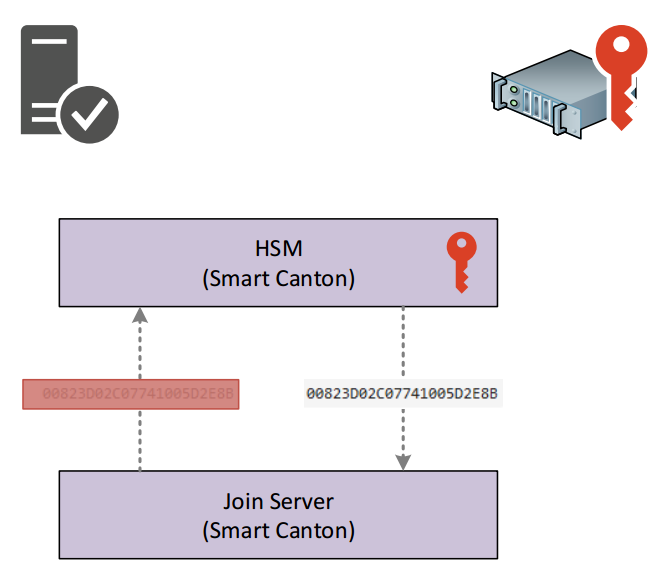
\includegraphics[width=0.5\textwidth]{Figures/Security/smartcanton/nshield_thales.png}
    \caption{Thales Nshield}
    \label{fig-nshield_thales}
\end{figure}



\subsubsection{\textit{Join Server}}

Pour faciliter la lecture des diagrammes du SmartCanton qui suivent, voici la légende des couleurs des clés utilisées : 
\begin{itemize}
    \item \textcolor[rgb]{0,0,1}{\textbf{Bleu}} : Application Key (AppKey);
    \item \textcolor[rgb]{1,0,0}{\textbf{Rouge}} : Application Session Key (AppSKey);
    \item \textcolor[rgb]{1,0.8,0}{\textbf{Orange}} : Network Session Key (NwkSKey).\\
\end{itemize}

\begin{figure}[ht!]
    \centering
    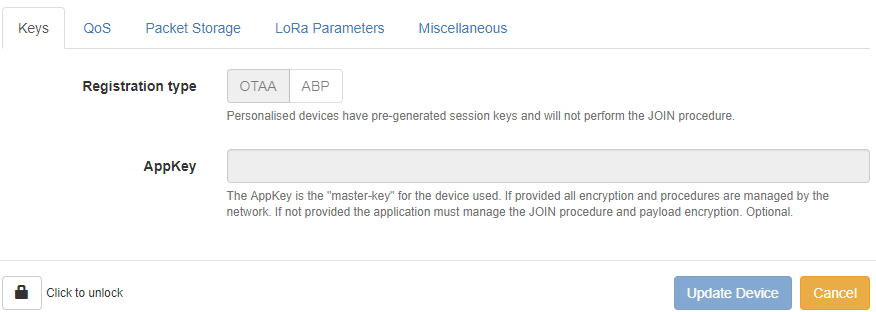
\includegraphics[width=0.55\textwidth]{Figures/Security/smartcanton/orbiwise_no_appkey.png}
    \caption{Périphérique enregistré sur un réseau OrbiWise sans AppKey}
    \label{fig-orbiwise_no_appkey}
\end{figure}

La fédération des opérateurs implémentée dans le POC est présentée à la \cref{fig-federation_network}, celle-ci est une composante primordiale pour la couverture en réseau du canton et de la ville de Genève. Le réseau d'OrbiWise autorise la création d'un périphérique sans spécification d'AppKey (cf. \cref{fig-orbiwise_no_appkey}, contrairement à TTN et Swisscom où cela est impossible. Cette fédération nécessite la redirection des requêtes vers un \textit{Join Server} personnalisé. Ce \textit{Join Server} est directement connecté au HSM pour la gestion des clés (cf. \cref{fig-nshield_thales}).\\


\begin{figure}[ht!]
    \centering
    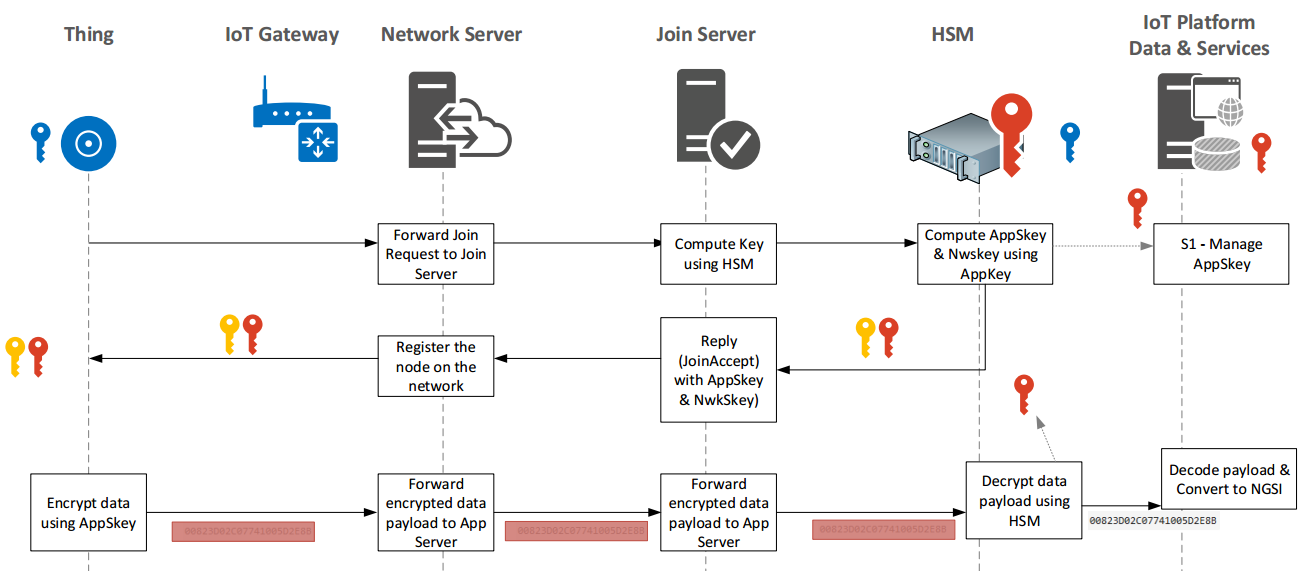
\includegraphics[width=1.0\textwidth]{Figures/Security/smartcanton/smartcanton_joinserver_decrypt_hsm.png}
    \caption{Déchiffrement des données par le HSM}
    \label{fig-smartcanton_joinserver_decrypt_hsm}
\end{figure}


OrbiWise équipe son infrastructure d'origine avec deux composants: un \textit{Network Server} (NST) pour la gestion du réseau et un Data Access Sub-System (DASS) qui équivaut à un \textit{Application Server} pour la récupération des données. Le \textit{Join Server} du SmartCanton travaille en tandem avec le Network Server d'OrbiWise pour récupérer les paquets qui sont envoyés par des périphériques inconnus au réseau d'OrbiWise. La \cref{fig-smartcanton_joinserver_decrypt_hsm} décrit la séquence complète de connexion d'un nouveau périphérique sur le réseau. Voici les points clés à retenir lors de la séquence de connexion à un partenaire du POC SmartCanton : 
\begin{enumerate}
    \item Le périphérique envoie un \textit{Join Request} sur le réseau.
    \item La \textit{gateway} de l'opérateur partenaire le récupère et l'envoi au \textit{Network Server} de l'opérateur.
    \item Le \textit{Network Server}, génère un AppNonce et l'envoi, conjointement à la demande de \textit{Join Request}, au \textit{Join Server} du SmartCanton.
    \item Le \textit{Join Server} identifie le périphérique comme étant autorisé à rejoindre le réseau et demande au HSM de créer les clés de sessions pour ce dernier. Une copie des clés est conservée à l'intérieur du HSM.
    \item Le Join Server construit et chiffre le Join Accept et le renvoi au Network Server accompagné de la NwkSKey.
    \item Le \textit{Network Server} \textit{forward} le \textit{Join Accept} vers le périphérique et sauvegarde en local la NwkSKey pour les futures communications avec le périphérique.
\end{enumerate}


\subsubsection{Cheminement des données et répartition des clés}

Le POC SmartCanton a pensé à deux implémentations de déchiffrement en utilisant les clés : 
\begin{enumerate}
    \item le déchiffrement des données est géré directement par le HSM. Cette implémentation est celle visible sur la \cref{fig-smartcanton_joinserver_decrypt_hsm}.
    \item le déchiffrement des données est géré par la plateforme IoT, par exemple, dans un module FIWARE. Cette implémentation est quant à elle visible sur la \cref{fig-smartcanton_joinserver_decrypt_hsm}.
\end{enumerate}

\begin{figure}[ht!]
    \centering
    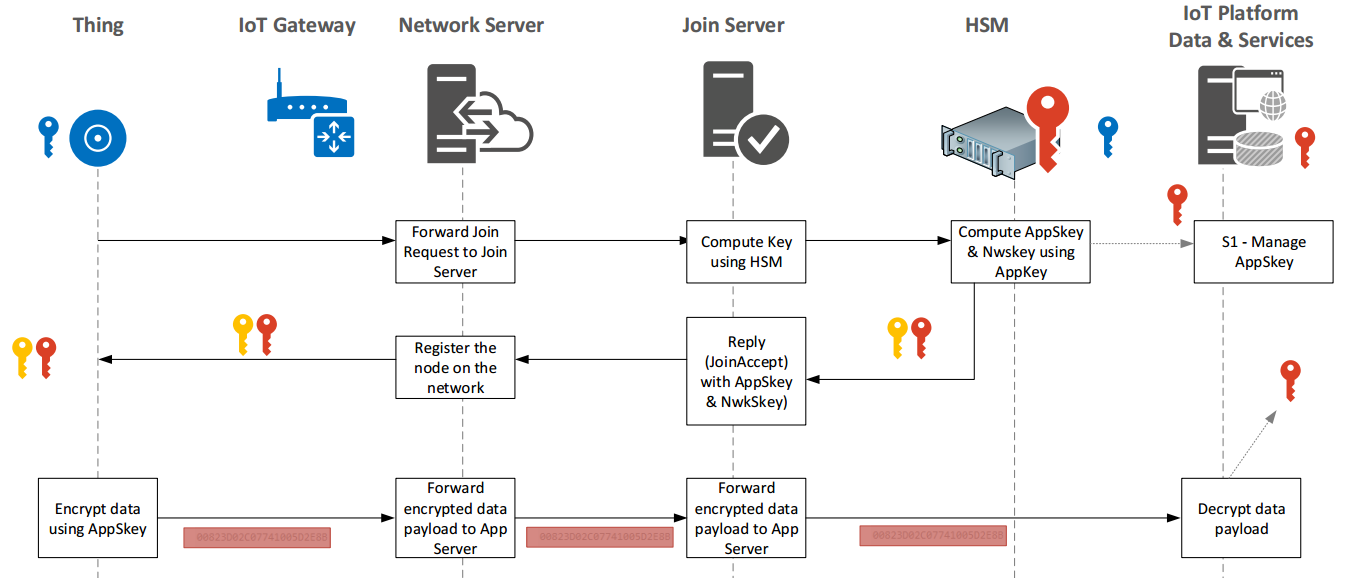
\includegraphics[width=1.0\textwidth]{Figures/Security/smartcanton/smartcanton_joinserver_decrypt_fiware.png}
    \caption{Déchiffrement des données par la plateforme IoT (FIWARE)}
    \label{fig-smartcanton_joinserver_decrypt_fiware}
\end{figure}


La \cref{fig-payload_journey} expose le cheminement complet d'un paquet de données produit par un périphérique (\textit{Thing}) jusqu'à l'application. On peut ainsi voir la répartition des différentes clés sur le schéma. La clé AppKey, la plus importante dans les connexions OTAA, est stockée en sécurité dans le HSM. La seule autre copie de cette clé est sur le périphérique. Le \textit{Network Server} de l'opérateur n'a accès qu'à la Network Session Key, il ne peut ainsi jamais déchiffrer les paquets de données. Cette implémentation reflète le principe qui est conseillé dans les recommandations énoncées à la \cref{sec-security_lorawan_recommendatiions}.

\begin{figure}[ht!]
    \centering
    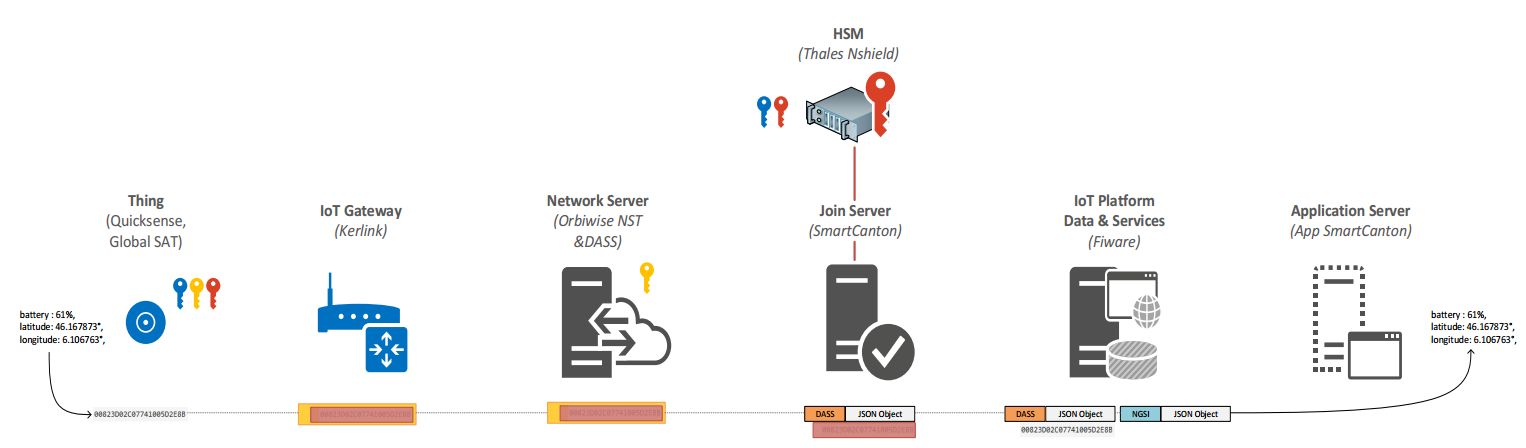
\includegraphics[width=1.0\textwidth]{Figures/Security/smartcanton/payload_journey.png}
    \caption{Cheminement des données depuis le périphérique jusqu'à l'application en utilisant le HSM pour le déchiffrement}
    \label{fig-payload_journey}
\end{figure}



